\documentclass{standalone}
\usepackage{tikz}

\definecolor{viridisblue}{RGB}{68,1,84}
\definecolor{viridisyellow}{RGB}{253,231,37}
\definecolor{viridisgreen}{RGB}{35,138,141}

\begin{document}

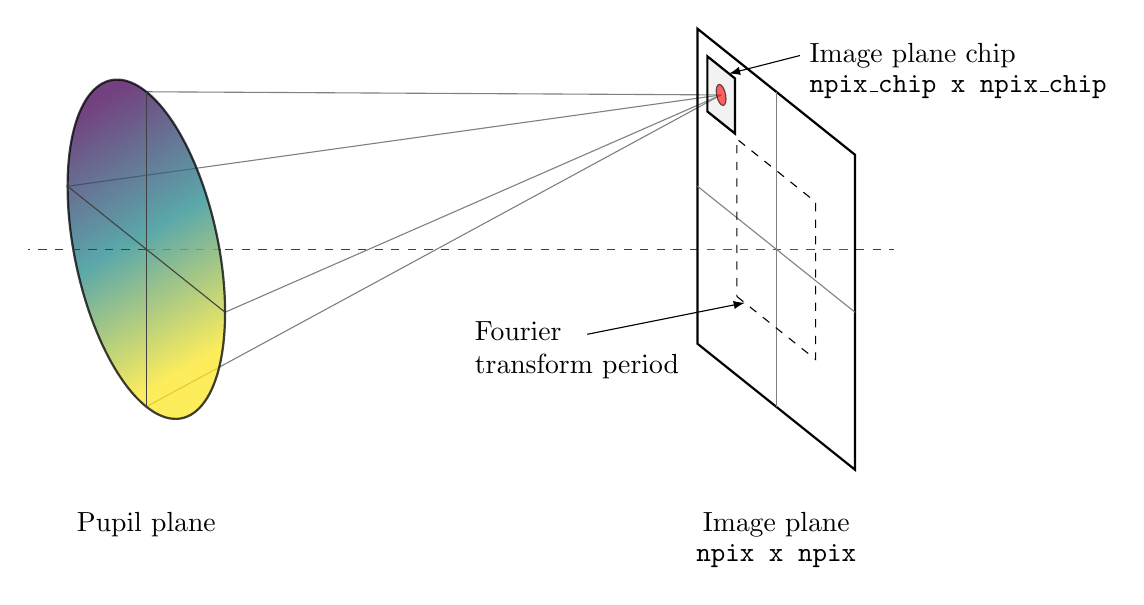
\begin{tikzpicture}[z={(1cm,0cm)},x={(0.5cm,-0.4cm)}, y={(0cm,1cm)}, scale=1]

    % constants
    \def\zimg{8}

    % coordinate system
    \coordinate (0) at (0,0,0);
    \coordinate (2) at (0,0,\zimg);

    % optical axis
    \draw[dashed, color=gray] (0) -- +(0,0,1);
    \draw[dashed, color=darkgray] (0,0,1) -- (0,0,9.5);


    % Aperture plane
    \draw[color=gray] (-2,0,0) -- (-1.4,1.4,\zimg);
    \draw[color=gray] (2,0,0) -- (-1.4,1.4,\zimg);
    \draw[color=gray] (0,-2,0) -- (-1.4,1.4,\zimg);
    \draw[color=gray] (0,2,0) -- (-1.4,1.4,\zimg);

    \draw[thick, shade, shading=axis, left color=viridisblue, right color=viridisyellow, middle color=viridisgreen,
    shading angle=30, opacity=0.75] (0,0) circle [radius=2];
    \draw[color=darkgray] (-2,0,0) -- (2,0,0);
    \draw[color=darkgray] (0,-2,0) -- (0,2,0);

    \draw[dashed, color=darkgray] (0) -- +(0,0,-1.5);  % left side of optical axis

    \node [align=left] at (0,-3.5,0) {Pupil plane};

    % Observation plane
    \draw [thick,fill=white,fill opacity=0.1] (-2,-2,\zimg) -- (2,-2,\zimg) -- (2,2,\zimg) -- (-2,2,\zimg) -- cycle;
    \draw[color=gray] (-2,0,\zimg) -- (2,0,\zimg);
    \draw[color=gray] (0,-2,0\zimg) -- (0,2,\zimg);

    \draw [thick,fill=gray,fill opacity=0.1] (-1.75,1.75,\zimg) -- (-1.75,1.05,\zimg) -- (-1.05,1.05,\zimg) -- (-1.05,1.75,\zimg) -- cycle;

    \draw[latex-] (-1.2,1.75,\zimg) -- (-1.4,1.9,9);
    \node [align=center, right] at (-1.4,1.9,9) {Image plane chip};
    \node [align=center, right] at (-1.4,1.5,9) {\texttt{npix\_chip x npix\_chip}};


    \draw[dashed] (-1,-1,\zimg) -- (1,-1,\zimg) -- (1,1,\zimg) -- (-1,1,\zimg) -- cycle;

    % Fourier transform period
    \draw[latex-] (-0.8,-1,\zimg) -- (-0.8,-1.4,6);
    \node [align=center, left] at (-0.8,-1.6,7.5) {\begin{tabular}{l} Fourier\\ transform period \end{tabular}};

    \node [align=center] at (0,-3.5,\zimg) {Image plane};
    \node [align=center] at (0,-3.9,\zimg) {\texttt{npix x npix}};


    % psf location
    \draw[fill=red, opacity=0.6] (-1.4,1.4,\zimg) circle [radius=0.125];

\end{tikzpicture}

\end{document}
